\documentclass[a4paper,12pt]{article}

% don't forget the document class, generally : \documentclass[a4paper,12pt]{article}

\usepackage[utf8]{inputenc}
\usepackage[french]{babel}
\usepackage{graphicx}
\usepackage{gensymb}
\usepackage{amsmath}
\usepackage{float}
\usepackage{scrextend}
\usepackage{caption} 
\usepackage{siunitx}
\usepackage{enumitem}
\usepackage{amsthm}
\usepackage{fancyhdr}
\usepackage{amssymb}
\usepackage{wrapfig}
\usepackage{geometry}
\usepackage{standalone}
\usepackage{import}
\usepackage[usenames, dvipsnames]{color}

 \usepackage{biblatex} % manages bibliography and references
\addbibresource{sample.bib}


\geometry{hmargin=1in, vmargin=1in}

 \newenvironment{absolutelynopagebreak}
 {\par\nobreak\vfil\penalty0\vfilneg
 \vtop\bgroup}
 {\par\xdef\tpd{\the\prevdepth}\egroup
 \prevdepth=\tpd}
 
 \pagestyle{fancy}                        
\fancyhf{}                               
\fancyhf[HL]{Application des maths}                
\fancyhf[HR]{Géométrie euclidienne}             
\fancyhf[FC]{\thepage/\pageref{Lastpage}}
 
\newtheorem{definition}{Définition}[section]
\newtheorem{theorem}{Théorème}
\newtheorem{corollary}{Corollaire}[theorem]
\newtheorem{lemma}[theorem]{Lemme}
\newtheorem*{hyp}{Hypothèse}
\newtheorem*{concl}{Conclusion}
\newtheorem*{remark}{Remarque}

\captionsetup{format=default,labelformat=simple,labelsep=colon,
justification=justified,font={sf,small},labelfont=bf,
textfont=default} 



\begin{document}

\pagebreak
\subsection{Théorème de la transversale}
\begin{theorem}\label{th:transversale}
Si deux droites $d$ et $d'$ ayant $e$ comme transversale ont une paire d'angles alternes-internes, alternes-externes ou correspondant isométriques, alors ces deux droites sont isométriques.\\
Aussi, si l'on considère la transversale $e$ à deux droites $d$ et $d'$ parallèles, alors une paire d'angle est isométrique lorsque ces angles sont: alternes-internes, alternes-externes ou  correspondants.
\end{theorem}
\begin{proof}
Nous considérons deux droites $d$ et $d'$ qui on $e$ comme transversale.
\begin{figure}[H]
    \centering
    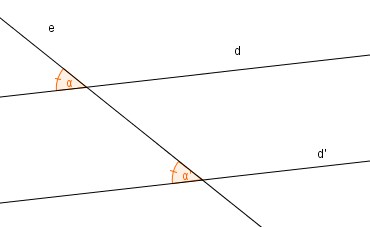
\includegraphics[scale=1]{schema/Transversale.PNG}
\end{figure}


\begin{hyp}
     $d$, $d'$ et $e$ sont trois droites,
     $\alpha$ et $\alpha'$ sont correspondants et
     $\alpha \equiv \alpha'$
 \end{hyp}
 \begin{concl}
     $d \parallel d'$
 \end{concl}
 En considérant l'hypothèse, il existe deux cas possibles:
 \begin{enumerate}
     \item $d$ et $d'$ se coupent en un point r
     \item $d$ et $d'$ sont parallèles
 \end{enumerate}
 Il nous faut démontrer que le cas 1) est faux et que le deuxième cas est le seul possible.\\
 Supposons que $d$ et $d'$ se coupent en un point r, il y a alors deux cas de figure possibles:
 \begin{enumerate}[label=\emph{\alph*}.]
  \item $\alpha'$ est à l'intérieur du triangle $\triangle pp'r$ et $\alpha$ est un angle externe. Par conséquent, grâce au théorème de l'angle externe, on sait que $\alpha>\alpha'$, ce qui est absurde. Donc il est impossible que d et d' se croisent et que $\alpha$ ou $\alpha'$ soient à l'intérieur du triangle $\triangle pp'r$.
  
    \begin{figure}[H]
        \centering
        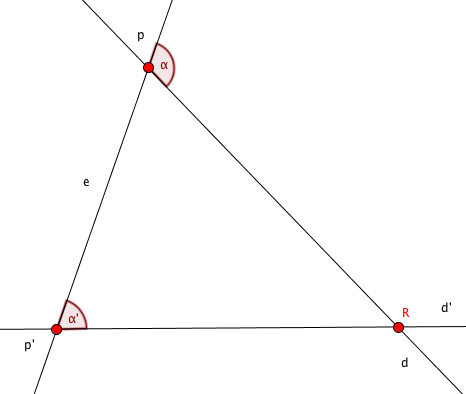
\includegraphics[scale=0.5]{schema/Transversale_3.png}
    \end{figure}
  
  
  \item Les angles $\alpha$ et $\alpha'$ sont à l'extérieur du triangle $\triangle pp'r$. Dans ce cas-là, par l'isométrie de deux angles opposés par le sommet (sous-section 6.7), on se retrouve dans le même cas qu'en a). Donc $\alpha$ et $\alpha'$ ne peuvent pas être à l'extérieur du triangle $\triangle pp'r$.
  
  
  \begin{figure}[H]
    \centering
    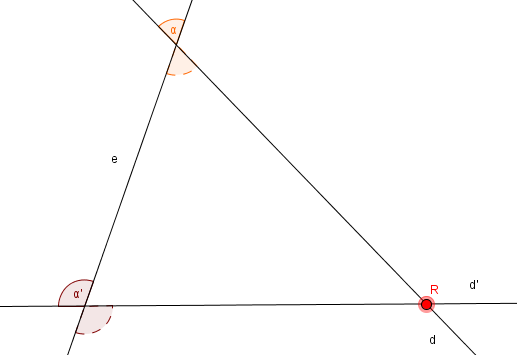
\includegraphics[scale=0.7]{schema/Transversale_2.PNG}
\end{figure}

  
 \end{enumerate}
 Le seul cas possible est donc le cas 2, $d$ et $d'$ sont parallèles.
\end{proof}

\begin{proof}
Nous considérons deux droites $d$ et $d'$ qui on $e$ comme transversale.

 \begin{figure}[H]
    \centering
    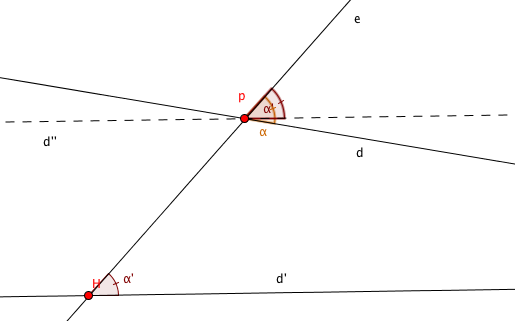
\includegraphics[scale=0.6]{schema/Transversale_4.png}
\end{figure}


\begin{hyp}
     $d$, $d'$ et $e$ sont trois droites,
     $\alpha$ et $\alpha'$ sont correspondants et
     $d \parallel d'$
 \end{hyp}
 \begin{concl}
     $\alpha \equiv \alpha'$
 \end{concl}
 Nous construisons la droite $d''$ qui passe par $p$ en reportant l'angle $\alpha'$. Grâce à la première partie de la démonstration, nous déduisons que d' est parallèle à d''. Donc, comme d' et d'' sont parallèles et qu'elles croisent e au point p, ces deux droites sont confondues (axiome des parallèles). On en conclu que $\alpha \equiv \alpha'$.
\end{proof}

\end{document}